\documentclass[a4paper,10pt,english]{article}
\usepackage[utf8]{inputenc}
\usepackage[english]{babel}
\usepackage{amsmath,graphicx,varioref,verbatim,amsfonts,geometry}
\usepackage[usenames,dvipsnames,svgnames,table]{xcolor}
\usepackage[colorlinks=false]{hyperref}

\setlength{\parindent}{0mm}
\setlength{\parskip}{1.5mm}

\usepackage{textcomp}
\definecolor{listinggray}{gray}{0.9}
\definecolor{lbcolor}{rgb}{0.9,0.9,0.9}

\usepackage{listings}

\lstdefinelanguage{python}
{
	morekeywords={print,abs,for,def,if,while,do,break,return,from,import,try,except,else,elif},
	sensitive=false,
	morecomment=[l]{\#}
}

\lstset{language=python,
	backgroundcolor=\color[rgb]{.95,.95,.95},
	numbers=left,xleftmargin=10pt,
	numberstyle=\tiny,stepnumber=1,numbersep=5pt,
	stringstyle=\color{red},
	basicstyle=\footnotesize \ttfamily,
	keywordstyle=\color{blue},
	commentstyle=\color{green},
	basewidth=0.60em,
	showstringspaces=false,
	captionpos=b,
	frame=single
}

\renewcommand{\thesubsection}{\roman{subsection}}
\renewcommand{\thesection}{\alph{section}}

\title{FYS-MEK1110 - Mandatory assignment 5}
\author{William Dugan}

\begin{document}

\maketitle

\section{} \label{a}
\begin{figure}[h!]
	\centering
	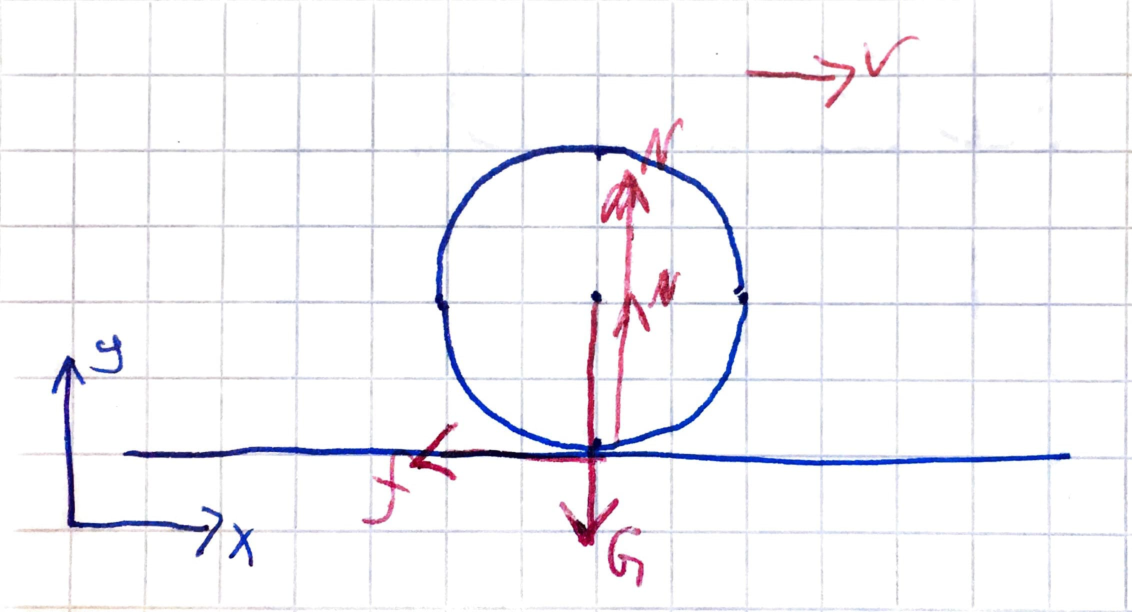
\includegraphics[scale=0.5]{freebodydiagram.pdf}
	\caption{Free body diagram of ball.}
	\label{fig:freebodydiagram}
\end{figure}

\section{} \label{b}
Since the two forces acting in y direction, we can use the equation of motion with constant acceleration to find the vertical position and vertical component of velocity. 
\begin{align*}
	\sum F_y &= m a_y \\
	N + G &= m a_y \\
	a_y &= \frac{N_0}{m} - g
\end{align*}
We can insert this into the equation of motion and get
\begin{align}
	v_y (t) &= v_{0, y} + \left( \frac{N_0}{m} - g \right) t \\
	y (t) &= R + v_{0, y} t + \frac{1}{2} \left( \frac{N_0}{m} - g \right) t^2
\end{align}

\section{} \label{c}
The time before ball changes direction is the time when the vertical velocity is zero.
\begin{align*}
	v_y (t_1) &= v_{0, y} + \left( \frac{N_0}{m} - g \right) t_1 \\
	\implies t_1 &= -\frac{v_{0, y}}{N_0/m - g} = -\frac{v_{0, y} m}{N_0 - mg}
\end{align*}
Since the forces acting on the ball is conservative, the time while the ball is in contact with the floor is
\begin{align*}
	t_c = 2 t_1 = -\frac{2v_{0, y} m}{N_0 - mg}
\end{align*}

\section{} \label{d}
To find the horizontal component of the velocity of the ball we can once again use the equation of motion with constant acceleration. The only force acting in x-direction is the friction force.
\begin{align*}
	\sum F_x &= m a_x \\
	\implies a_x &= -\frac{\mu N}{m}
\end{align*}
Inserting into the equation of motion we get
\begin{align}
	v_x (t) = v_{0, x} - \frac{\mu N}{m} t
\end{align}
The horizontal component of velocity right after the collision is
\begin{align*}
	v_x (t_1) &= v_{0, x} + \frac{\mu N}{m} \frac{2v_{0, y} m}{N_0 - mg} \\
	&= v_{0, x} + v_{0, y} \frac{2 \mu}{(1-mg/N_0)}
\end{align*}
We note that $v_{1, x} < v_{0, x}$ since $v_{0, y} < 0$.

\section{} \label{e}
To find the angular velocity as a function of time we use the two equations for torque.
\begin{align}
	\tau &= I \alpha \\
	\tau &= \vec{F} \times \vec{r} = |F| \cdot |r| \sin\theta
\end{align}
If we rearrnge the equations above to solve for angular acceleration, we get
\begin{align*}
	\alpha = \frac{F_x r}{I} = - \frac{3 \mu N}{2 m r}
\end{align*}
where we have used that the driving force acts perpendicular to the direction of travel. Since this acceleration is constant, we can use the equation of rotational motion with constant angular acceleration.
\begin{align}
	\omega (t) = - \frac{3 \mu N_0}{2 m r} t
\end{align}
The angular velocity right after the collision is
\begin{align*}
	\omega (t_1) = \frac{3 \mu N_0}{2 m r} \frac{v_{0, y} m}{N_0 - mg} = \frac{3 \mu v_{0, y}}{r (1 - mg/N_0)}
\end{align*}
Since $v_{0, y} < 0$ the rotation of the ball is clockwise.

\section{} \label{f}
The work done by the friction force is not independent of the path taken, hence mechanical energy is not conserved.

\section{} \label{g}
We will now model the norml force as 
\begin{align}
	N = k (R - y)^{3/2}
\end{align}
where $y < R$. We repeat the procedure we did earlier to find the acceleration.
\begin{align*}
	\sum F_x &= m a_x 		& 	\sum F_y &= m a_y \\
	-\mu N &= m a_x 		& 	G + N &= m a_y \\
	a_x &= -\frac{\mu N}{m} & 	a_y &= \frac{N}{m} - g
\end{align*}

\section{} \label{h}
To find the angular acceleration $a_z$ we use
\begin{align}
	\alpha = \frac{d \omega}{dt}.
\end{align}
Using this, we can find $a_z$.
\begin{align*}
	a_z = \frac{d \omega}{dt} = \frac{3 \mu N}{2 m r} = \frac{3 \mu k (R-y)^{3/2}}{2 m r}
\end{align*}

\newpage

\section{} \label{i}
\lstinputlisting{integration.py}

\begin{figure}[h!]
	\centering
	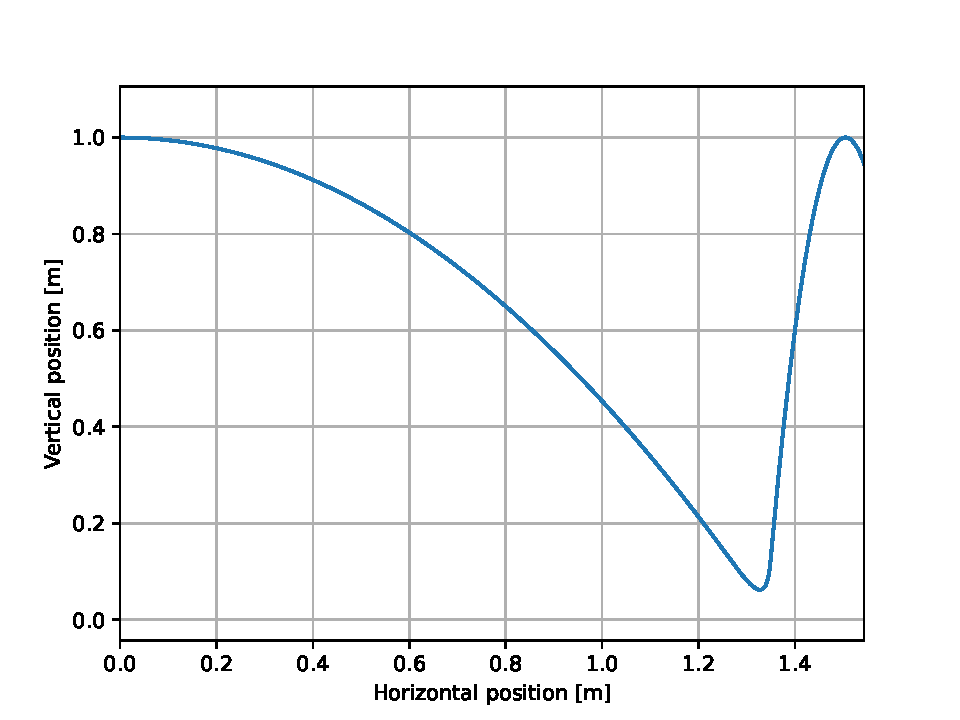
\includegraphics[scale=0.7]{position.pdf}
	\caption{Plot of horizontal and vertical position over time.}
	\label{fig:dist}
\end{figure}

\begin{figure}[h!]
	\centering
	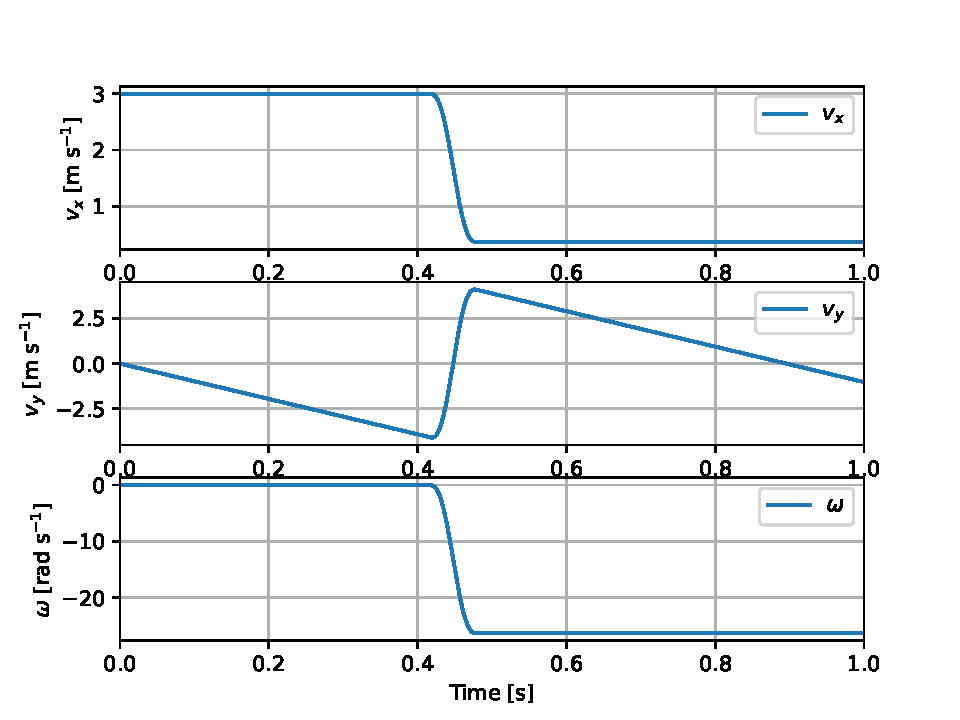
\includegraphics[scale=0.7]{velocities.pdf}
	\caption{Plot of linear and angular velocity over time.}
	\label{fig:vel}
\end{figure}

From figure \ref{fig:dist} we see that the ball bounces back to the same height as before the collision. This confirms the result in section \ref{c}. It also shows that translational momentum is conserved. We also observe that $y_{text{min}} < R$ which means that our assumption that the ball does not deform during the collision is somewhat unprecise. The ball will continue to rotate with constant angular velocity after the collision.

\section{}
Our numerical simulation is not an accrurate representation of a ball hitting the ground as we assume that it is an elastic collision. This could be improved if we modeled the normal force differently and in a way that makes it non-conservative. A final thought is that since we assume the ball does not deform, we also underestimate the effect of friction, as we assume it only has a single contact point. This would not be the case since the ball deforms and the contact surface increase.

\end{document}